\documentclass[11pt,letterpaper]{article}
\usepackage[utf8]{inputenc}
\usepackage[T1]{fontenc}
\usepackage[spanish,es-nodecimaldot]{babel}
\usepackage{lmodern}
\usepackage[margin=2cm]{geometry}
\usepackage{graphicx}
\usepackage{booktabs}
\usepackage{longtable}
\usepackage{array}
\usepackage{enumitem}
\usepackage{xcolor}
\usepackage{hyperref}
\usepackage{caption}

\hypersetup{
  colorlinks=true,
  linkcolor=blue!50!black,
  urlcolor=blue!50!black,
  pdftitle={Practica 8 - Pruebas de caja negra de GameStore},
  pdfauthor={},
  pdfsubject={Evaluacion de calidad de software}
}
\setlength{\parskip}{0.45em}
\setlength{\parindent}{0pt}
\renewcommand{\arraystretch}{1.2}
\newcommand{\aprobado}{\textbf{APROBADO}}
\newcommand{\bloqueado}{\textbf{NO VERIFICADO}}

\begin{document}

\pagenumbering{roman}
\begin{titlepage}
  \centering
  \vspace*{2cm}
  {\Large Evaluación de calidad de software\par}
  \vspace{0.5cm}
  {\huge\bfseries PRACTICA 8\par}
  \vspace{0.3cm}
  {\LARGE Pruebas de caja negra (Black Box Testing)\par}
  \vspace{1.5cm}
  {\Large Proyecto: GameStore -- catálogo de videojuegos\par}
  \vfill
  \begin{tabular}{rl}
    Alumno: & \rule{9cm}{0.4pt}\\[0.8cm]
    Asignatura: & \rule{9cm}{0.4pt}\\[0.8cm]
    Docente: & \rule{9cm}{0.4pt}\\[0.8cm]
    Fecha: & 23 de octubre de 2026
  \end{tabular}
  \vfill
  {\large Evidencia automatizada y visual\par}
\end{titlepage}

\pagenumbering{arabic}
\tableofcontents
\newpage

\section{Objetivo y alcance}
Evaluar, desde las entradas y salidas observables, las funciones disponibles en GameStore:
catálogo, búsqueda, autenticación y segundo factor (2FA), control de acceso, carrito y manejo de
errores. Se prepararon pruebas automatizadas de componentes/servicios Angular con datos
controlados, además de capturas del sitio ejecutándose localmente.

La suite implementa 19 casos de comportamiento identificados con códigos \texttt{RF-*}, que
coinciden directamente con los identificadores de los requisitos de este informe. Los
casos no hacen llamadas a cuentas ni datos reales: los servicios de backend se sustituyen por
dobles de prueba y la persistencia evaluada en el carrito corresponde a \texttt{localStorage}.
Esto permite repetir las pruebas sin modificar información de producción.

\textbf{Alcance no cubierto:} no se pudo validar la integración real con Supabase, las operaciones
CRUD remotas, ni una transacción monetaria. La API remota no respondió durante la inspección del
navegador y el servicio local no se inició. Por ello, los resultados de las pruebas aisladas no se
interpretan como certificación del backend.

\section{Inventario de funcionalidades}
\begin{itemize}[leftmargin=1.5em]
  \item Inicio e información del sitio con navegación hacia el catálogo y acceso.
  \item Catálogo de videojuegos con título, plataforma, precio y stock; búsqueda por título o
  plataforma.
  \item Registro e inicio de sesión, flujo de configuración 2FA y verificación TOTP.
  \item Carrito con adición, consolidación de artículos repetidos, cantidades, cálculo del total,
  eliminación y vaciado. El estado se guarda localmente para visitantes y se sincroniza por API
  cuando hay sesión.
  \item Perfil de usuario y registro biométrico, sujeto a compatibilidad del navegador.
  \item Panel administrativo para inventario y usuarios, con operaciones de alta, modificación,
  baja lógica y eliminación.
  \item Interceptor HTTP que informa fallas de red.
\end{itemize}

No se encontró una especificación funcional externa o criterios de aceptación previos. Por tanto,
los requisitos siguientes se derivan de la interfaz, sus validaciones y el comportamiento
implementado. Deben confirmarse con el responsable del producto antes de considerarse la
especificación oficial.

\section{Requisitos verificables y criterios de aceptación}
Cada criterio indica una condición observable y medible. El resultado \aprobado{} significa que
el caso automatizado pasó con sus datos controlados; no implica que una operación remota esté
probada.

\small
\begin{longtable}{>{\raggedright\arraybackslash}p{1.5cm}
                  >{\raggedright\arraybackslash}p{3.1cm}
                  >{\raggedright\arraybackslash}p{7.6cm}
                  >{\raggedright\arraybackslash}p{2.5cm}}
\toprule
\textbf{ID} & \textbf{Requisito / entrada} & \textbf{Criterio de aceptación medible} &
\textbf{Resultado}\\
\midrule
\endfirsthead
\toprule
\textbf{ID} & \textbf{Requisito / entrada} & \textbf{Criterio de aceptación medible} &
\textbf{Resultado}\\
\midrule
\endhead
RF-01 & Mostrar catálogo con dos juegos de prueba. &
Se muestran exactamente 2 tarjetas con título y precio correspondientes a los datos recibidos. &
\aprobado{}\\
RF-02 & Buscar \texttt{"  ELDEN  "}. &
La búsqueda ignora mayúsculas y espacios externos; queda exactamente 1 resultado: Elden Ring. &
\aprobado{}\\
RF-03 & Buscar \texttt{"switch"} y luego un texto inexistente. &
La plataforma Nintendo Switch produce 1 resultado; la consulta inexistente produce 0 tarjetas. &
\aprobado{}\\
RF-04 & Visitante selecciona agregar al carrito. &
Se navega a \texttt{/login} y no se invoca la operación de agregado. &
\aprobado{}\\
RF-05 & Usuario autenticado agrega Elden Ring. &
El carrito recibe ID, título, plataforma, precio e imagen correctos, con cantidad inicial igual a 1. &
\aprobado{}\\
RF-06 & Enviar contraseña de 5 caracteres. &
El inicio de sesión no se invoca y se muestra el mensaje de longitud mínima de 6 caracteres. &
\aprobado{}\\
RF-07 & Iniciar sesión con correo en mayúsculas y espacios. &
El servicio recibe el correo en minúsculas y sin espacios, y la interfaz avanza al paso 2FA. &
\aprobado{}\\
RF-08 & Registro con contraseñas diferentes. &
No se llama al registro y se muestra el mensaje de que las contraseñas no coinciden. &
\aprobado{}\\
RF-09 & Backend rechaza credenciales. &
Se muestra el mensaje de correo o contraseña incorrectos; el error no se interpreta como acceso. &
\aprobado{}\\
RF-10 & Introducir un código TOTP inválido. &
Se rechaza el código, se limpia la entrada y no se guarda la marca de 2FA aprobado. &
\aprobado{}\\
RF-11 & Abrir ruta protegida sin sesión. &
El guard deniega el acceso y solicita navegación a \texttt{/login}. &
\aprobado{}\\
RF-12 & Abrir ruta con sesión, pero sin marca 2FA. &
El guard deniega el acceso y solicita navegación a \texttt{/login}. &
\aprobado{}\\
RF-13 & Abrir ruta con sesión y 2FA aprobado. &
El guard permite la navegación y no redirige al inicio de sesión. &
\aprobado{}\\
RF-14 & Cliente abre el panel administrativo. &
Se muestra acceso restringido y no se muestran los controles de alta/modificación del admin. &
\aprobado{}\\
RF-15 & Agregar dos veces el mismo producto (precio \$40). &
Se conserva un solo registro con cantidad 2, total \$80 y cantidad 2 en \texttt{localStorage}. &
\aprobado{}\\
RF-16 & Reducir a cero la cantidad del artículo. &
El artículo desaparece del carrito y el arreglo persistido queda vacío. &
\aprobado{}\\
RF-17 & Reinicializar el carrito con un registro persistido. &
Se restaura 1 artículo y su total es \$40. &
\aprobado{}\\
RF-18 & Vaciar el carrito local. &
El total queda en \$0 y se elimina la clave \texttt{carrito} de \texttt{localStorage}. &
\aprobado{}\\
RF-19 & Falla de red HTTP con estado 0. &
Se muestra la alerta de servidor no disponible y se propaga el error original. &
\aprobado{}\\
\bottomrule
\end{longtable}
\normalsize

\subsection{Cobertura mínima solicitada}
\begin{itemize}[leftmargin=1.5em]
  \item Operaciones principales: RF-01, RF-03, RF-05, RF-15.
  \item Validaciones: RF-06, RF-08, RF-10 y RF-16.
  \item Persistencia/consistencia local: RF-15, RF-16, RF-17 y RF-18.
  \item Navegación y permisos: RF-04 y RF-11 a RF-14.
  \item Manejo de errores: RF-09 y RF-19.
\end{itemize}

\section{Ejecución y resultados}
Las pruebas se ejecutan desde \texttt{gamestore-frontend} con:
\begin{verbatim}
npm test -- --watch=false
npm run build
\end{verbatim}

Resultado de la suite: \textbf{31 pruebas aprobadas, 0 fallidas y 0 errores no controlados},
distribuidas en 11 archivos de prueba. De ellas, 19 corresponden a los requisitos de
comportamiento RF-01 a RF-19; las restantes cubren creación de componentes y limpieza del estado
de autenticación. La compilación de producción de Angular también finalizó correctamente.

Los escenarios usan dos videojuegos sintéticos (Elden Ring, PC, \$799; Tears of the Kingdom,
Nintendo Switch, \$1199) para probar lista y filtrado. Los datos no se escriben en Supabase. Las
capturas se tomaron en la aplicación local y se incluyen como evidencia de presentación, no como
evidencia de operación del backend.

\section{Evidencia visual}
\begin{figure}[htbp]
  \centering
  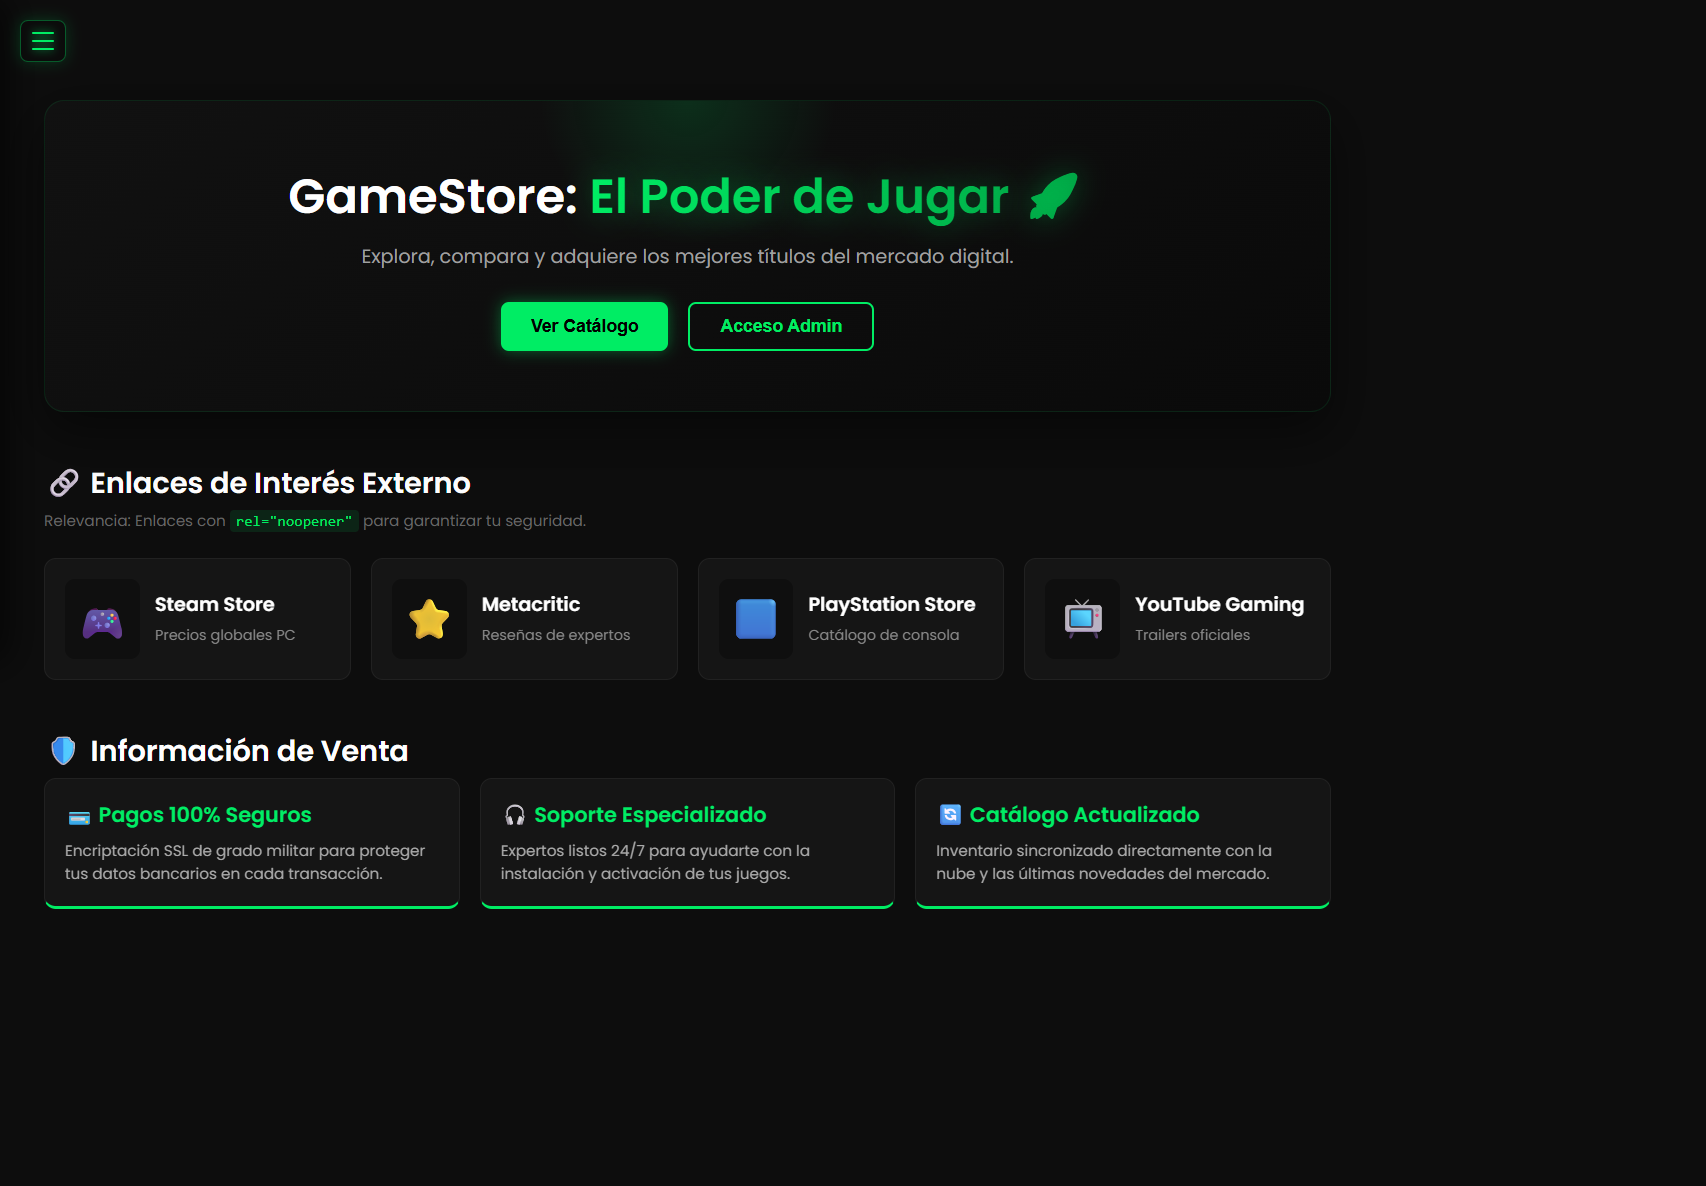
\includegraphics[width=0.92\textwidth,height=0.48\textheight,keepaspectratio]
  {evidencia/inicio.png}
  \caption{Pantalla de inicio cargada en el navegador local.}
  \label{fig:inicio}
\end{figure}

\begin{figure}[htbp]
  \centering
  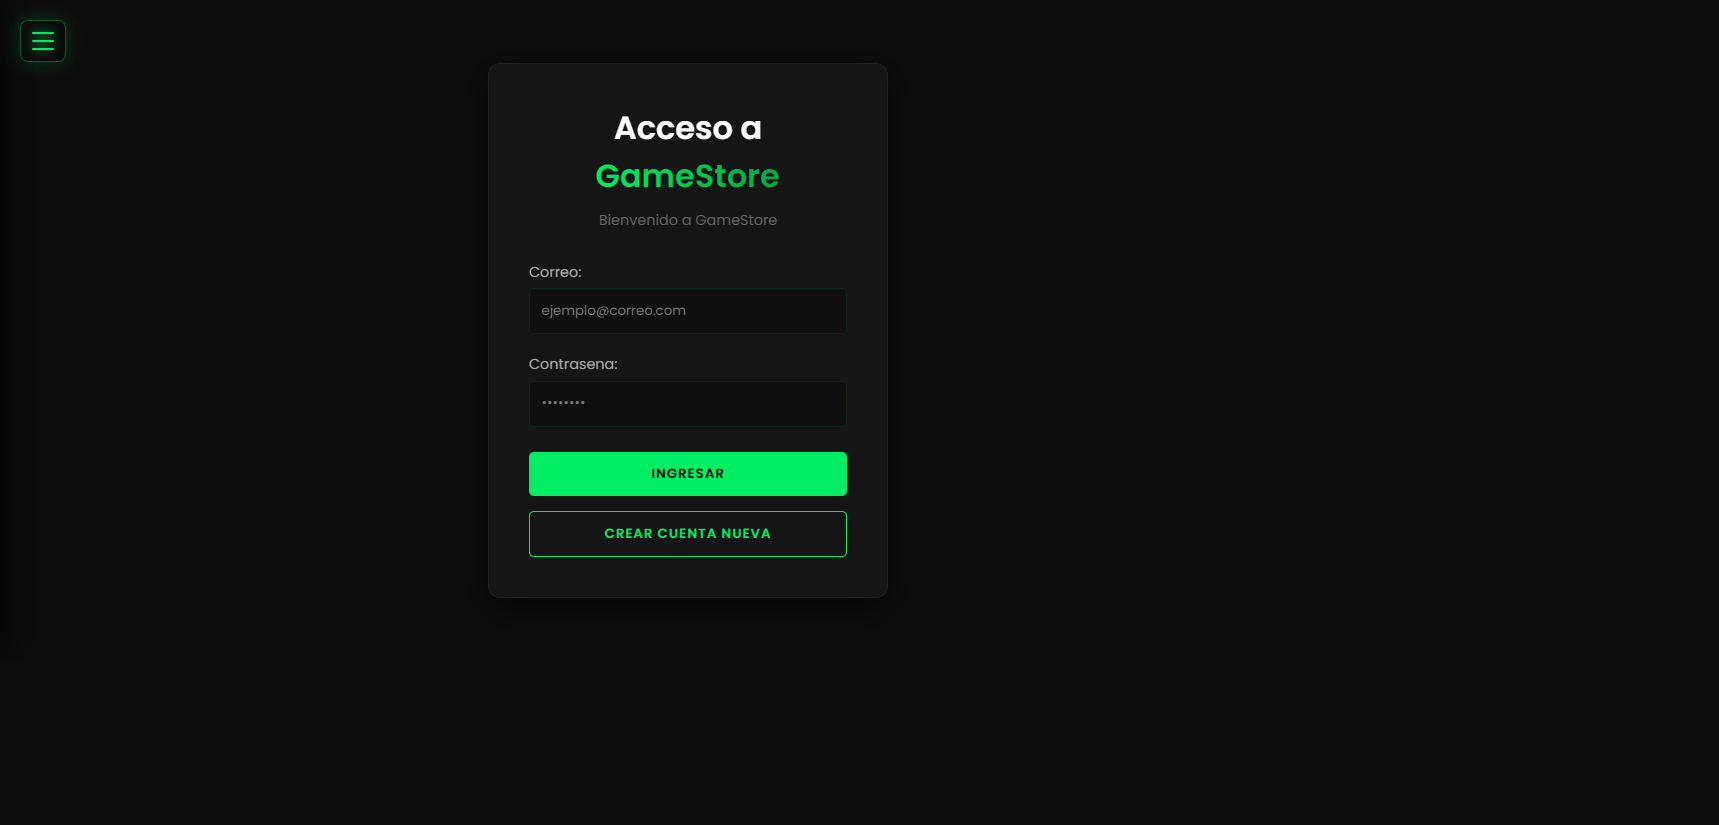
\includegraphics[width=0.78\textwidth,height=0.55\textheight,keepaspectratio]
  {evidencia/login.png}
  \caption{Formulario de acceso y opción de creación de cuenta.}
  \label{fig:login}
\end{figure}

\section{Requisitos pendientes por falta de entorno o información}
\begin{longtable}{>{\raggedright\arraybackslash}p{1.5cm}
                  >{\raggedright\arraybackslash}p{4.9cm}
                  >{\raggedright\arraybackslash}p{8.3cm}}
\toprule
\textbf{ID} & \textbf{Requisito no verificable} & \textbf{Motivo / evidencia requerida}\\
\midrule
\endfirsthead
\toprule
\textbf{ID} & \textbf{Requisito no verificable} & \textbf{Motivo / evidencia requerida}\\
\midrule
\endhead
NV-01 & Persistencia de catálogo, perfiles y carrito remoto. &
Requiere API y base Supabase de pruebas accesibles. La suite actual simula sus respuestas y solo
verifica el carrito local.\\
NV-02 & Alta, modificación, baja y eliminación reales de juegos y usuarios. &
Requiere cuenta administrativa de staging, datos semilla y verificación posterior en base de
datos; no se hicieron cambios destructivos a datos reales.\\
NV-03 & Autorización administrativa del lado del servidor. &
No se encontró middleware de autenticación/rol en \texttt{gamestore-backend/server.js}; las rutas
de gestión no deben confiar en que Angular oculte los controles. Se necesita prueba negativa
contra una API de staging tras implementar o confirmar esa protección.\\
NV-04 & Transacción de pago real y consistencia con el stock. &
No se dispuso de pasarela ni entorno de pago. El flujo visible de pago solo espera y muestra éxito;
no acredita un cobro, reserva de stock o recibo.\\
NV-05 & 2FA completo con secreto remoto y códigos válidos en el tiempo. &
Se probó el rechazo de un código TOTP; no se pudo comprobar la emisión/escaneo del QR, guardado
remoto, login completo o tolerancia de reloj en el backend.\\
NV-06 & Registro/verificación biométrica WebAuthn. &
Necesita dispositivo con autenticador de plataforma, credenciales y API disponible.\\
NV-07 & Criterios de negocio oficiales. &
No hay documento previo con reglas de precios, stock, cantidades máximas, transacciones o roles;
los requisitos de esta práctica se derivaron del producto implementado.\\
\bottomrule
\end{longtable}

\section{Defectos y riesgos para liberación}
\begin{enumerate}[leftmargin=1.7em]
  \item \textbf{Bloqueante para producción -- autorización de API pendiente.} El control de rol
  observado está en el cliente. La ausencia de middleware de autorización en las rutas del
  servidor significa que ocultar botones no prueba que un usuario cliente no pueda invocar
  operaciones administrativas directamente. Antes de liberar, proteger cada ruta y probar
  respuestas 401/403 con usuario no administrador.
  \item \textbf{Bloqueante si se anuncia venta en línea -- pago simulado.} El flujo presenta
  confirmación de pago sin evidencia de integración con procesador ni decremento/reserva de
  inventario. No aceptar como compra real hasta verificar el servicio transaccional, errores,
  idempotencia y consistencia de stock.
  \item \textbf{Defecto de interacción -- botón ``Ver detalles''.} En la tarjeta de catálogo se
  presenta un botón sin acción asociada observable. Definir el comportamiento esperado o retirar
  el control antes de liberar esa funcionalidad.
  \item \textbf{Manejo de error parcial.} El interceptor alerta en error de red, pero la carga del
  catálogo solo registra el fallo en consola; falta estado visible de error/reintento para el
  usuario.
  \item \textbf{Dependencia del backend no disponible.} En la sesión de evidencia el servicio
  remoto no respondió y el cliente cambió a localhost. No se pudo validar recuperación,
  persistencia ni CRUD remotos en ese entorno.
\end{enumerate}

\section{Conclusión y dictamen}
La evidencia respalda la aceptación \textbf{parcial del frontend como prototipo académico}: las
31 pruebas ejecutadas pasaron, se verifican búsqueda, validaciones, estado de carrito local,
reglas de navegación y algunas respuestas de error; además, la aplicación compila en modo
producción.

\textbf{No se recomienda aceptar la liberación productiva en el estado evaluado.} Permanecen sin
verificar la persistencia y el CRUD de backend, el cobro real y las autorizaciones administrativas
en servidor. Los riesgos NV-03 y NV-04 son bloqueantes para una tienda que gestione datos de
administración o anuncie ventas. Para un dictamen de aceptación completo se requiere repetir las
pruebas contra staging con datos sintéticos, credenciales por rol, API protegida y pasarela de
prueba.

\end{document}
